%%%
%%% HEADER
%%%

\documentclass[a4paper]{article}

\usepackage[utf8]{inputenc}
\usepackage[T1]{fontenc}
\usepackage[czech]{babel}
\usepackage{listings} 
\usepackage[pdfborder={1 0 0}]{hyperref} 
\usepackage{graphicx}
\usepackage{wrapfig}
\usepackage{subfig}
\usepackage{color}
\usepackage{xcolor}
\usepackage{amsmath}
\usepackage{caption}
\usepackage[a4paper,vmargin={35mm, 35mm}, hmargin={35mm, 35mm}]{geometry}
\usepackage[affil-it]{authblk} 
\usepackage{etoolbox}
\usepackage{lmodern}
\usepackage{titlesec}

%% colors
\definecolor{titleblue}{rgb}{0.02, 0.37, 0.55}
\definecolor{sectionblue}{rgb}{0.25, 0.44, 0.60}
\definecolor{subsectionblue}{rgb}{0.37, 0.59, 0.77}
\definecolor{gray}{rgb}{0.9,0.9,0.9}

%% mod title section
\makeatletter
% line hackity hack
\let\old@rule\@rule
\def\@rule[#1]#2#3{\textcolor{titleblue}{\old@rule[#1]{#2}{#3}}}
\renewcommand{\@maketitle}{
  % font family shortcuts ref: http://tex.stackexchange.com/a/25251
  \begin{flushleft}
  {\color{titleblue}
   \fontfamily{lmss}
   \fontsize{26}{0}
   \selectfont
   \@title
   }{}{}
  \end{flushleft}

  \noindent\makebox[\linewidth]{\rule{\textwidth}{0.1pt}}
  \par
  {\fontsize{1}{0}\@author} %authorhack
  \fontfamily{lmss}\fontsize{12}{0}\color{subsectionblue}\\
  \noindent\textit{Vedoucí týmu: Vojtěch Dlápal (dlapavoj, 107)}\\ \\
  \noindent\textit{Členové týmu: Jan Hoffman (hoffmja2, 107), Tomáš Duda (dudatom2, 106)}\\ \\
  \noindent\textit{Datum: \@date}
}
\makeatother

%% mod styles
\titleformat*{\section}{\LARGE\bfseries\sffamily\color{sectionblue}}
\titleformat*{\subsection}{\Large\bfseries\sffamily\color{subsectionblue}}
\titleformat*{\subsubsection}{\large\bfseries\sffamily\color{subsectionblue}}

%% mod listings
\DeclareCaptionFont{white}{\color{white}}
\DeclareCaptionFont{black}{\color{black}}
\DeclareCaptionFormat{listing}{\colorbox{gray}{\parbox{\textwidth}{#1#2#3}}}
\captionsetup[lstlisting]{format=listing,labelfont=black,textfont=black}


%%%
%%% DOCUMENT
%%%

\begin{document}

\title{MI-SPI 2016 — Domácí úkol č. 1}
\author{-} % authorhack
\date{\today}
\maketitle

%%
%% Úkol 1
%%

\section{Generování náhodného výběru a grafické ověřování jeho rozdělení [1,5b]}
\subsection{}
Vygenerujte $n = K*20$ náhodných hodnot z rozdělení $Exp(L)$ pomocí inverze distribuční funkce. Tj. do proměnné $u$ uložte $n$ náhodných rovnoměrně rozdělených hodnot v intervalu $(0,1)$ a pak do proměnné $x$ uložte jejich transformaci takovou, aby výsledný výběr $x$ byl z požadovaného rozdělení $Exp(L)$. Transformace bude inverze distribuční funkce rozdělení $Exp(L)$. Pozor, zde $L$ je intenzita rozdělení (rate), nikoliv jeho střední hodnota. Náhodné výběry generujeme pomocí funkcí $runif$, $rnorm$, $rexp$, apod.

\lstset{language = r, numbers=left, tabsize = 4, title=Řešení, basicstyle=\footnotesize}
\begin{lstlisting}[firstnumber=1]
K = 6 # Pocet znaku ve jmene Vojtech
L = 6 # Pocet znaku v prijmeni Dlapal
n = K * 20 # Pocet hodnot k vygenerovani
u = runif(n) # Generuji n nahodnych rovnomerne rozdelenych hodnot mezi 0 a 1
x = qexp(u, rate=L) # quantile function - inverze distribucni fce
\end{lstlisting}

\subsection{}
Vytvořte histogramy dat v $u$ a $x$. Histogram $x$ zobrazte spolu s grafem hustoty rozdělení $Exp(L)$. Histogram můžeme získat pomocí příkazu $hist()$ — pozor na parameter $probability=$. Graf hustoty lze přidat k histogramu příkazem $lines()$. Hustoty různých rozdělení lze získat pomocí funkcí $dunif$, $dnorm$, $dexp$, apod. Např. pro normální rozdělení se střední hodnotou m a směrodatnou odchylkou $s$ můžeme použít

\lstset{title=Tip}
\begin{lstlisting}
# Normal Distribution
xWidth = max(x) - min(x)
xGrid = seq(min(x) - 0.2 * xWidth, max(x) + 0.2 * xWidth, length = 30)
lines (xGrid, dnorm(xGrid, mean = m, sd = s), col = 'red', lw = 2, lty = 2)
\end{lstlisting}

\lstset{language = r, numbers=left, tabsize = 4, title=Řešení, basicstyle=\footnotesize}
\begin{lstlisting}[firstnumber=5]
# Histogram u
hist(u, probability = TRUE) # Parametr probability = normalizace
# Histogram x
xWidth=max(x) - min(x) # Interval generovanych hodnot
# Vygeneruji posloupnost hodnot z daneho intervalu
xGrid=seq(min(x) - 0.2 * xWidth, max(x) + 0.2 * xWidth, length(x))
hist(x, probability = TRUE) # Histogram x
# Spojeni bodu v grafu do krivky
lines(xGrid, dexp(xGrid, rate = L), col = 'red', lw = 2, lty = 2)
\end{lstlisting}

\begin{figure}[h]
\begin{center}
	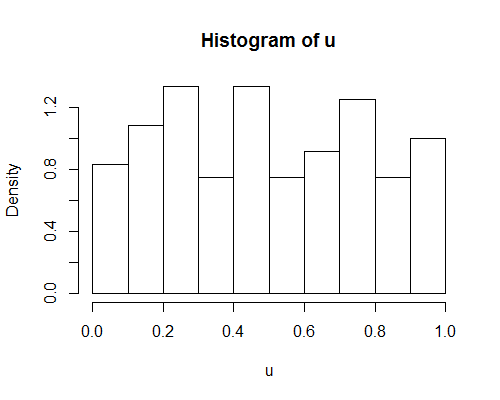
\includegraphics{hist_u.png}
\end{center}
\end{figure}

\begin{figure}[h]
\begin{center}
	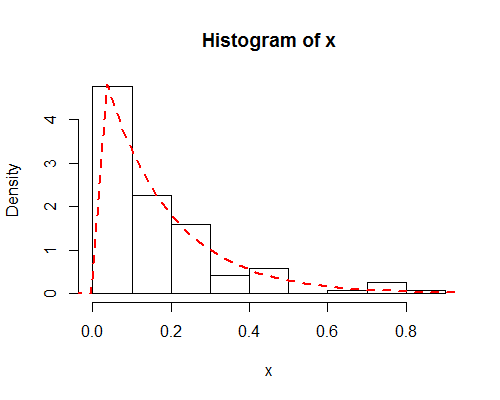
\includegraphics{hist_x.png}
\end{center}
\end{figure}

\subsection{}
Vygenerujte graf empirické distribuční funkce pro data z $x$ spolu s grafem distribuční funkce rozdělení $Exp(L)$. Graf empirické distribuční funkce můžeme získat pomocí příkazu $plot(ecdf(x), verticals=TRUE, do.points = FALSE, main=„Titulek grafu“)$. Grafy teoretické distribuční funkce přidáme opět pomocí příkazu $lines()$, kde ale $dunif$, $dnorm$ a $dexp$ nahradíme pomocí $punif$, $pnorm$ a $pexp$.

\lstset{language = r, numbers=left, tabsize = 4, title=Řešení, basicstyle=\footnotesize}
\begin{lstlisting}[firstnumber=14]
plot(ecdf(x), verticals = TRUE, do.points = FALSE, main = "Porovnani ECDF a CDF rozdeleni Exp(L)", ylab = "cdf(x)")
lines(xGrid, pexp(xGrid, rate = L), col = 'red', lw = 2, lty = 2)
\end{lstlisting}

\begin{figure}[h]
\begin{center}
	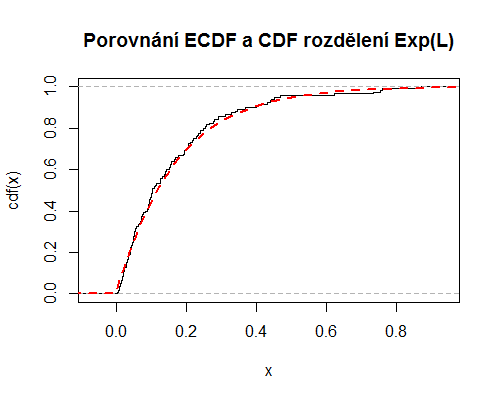
\includegraphics{ecdf.png}
\end{center}
\end{figure}

\subsection{}
Vygenerujte „pravděpodobnostní papír“ pro porovnání rozdělení dat $x$ s rozdělením $Exp(L)$. Použít můžeme $qqplot(x, y); abline(0,1, col='red', lwd=2)$, kde $x$ obsahuje data a $y$ nový náhodný výběr z rozdělení, se kterým data porovnáváme. Např. $y=rexp(1000, rate=1/m)$.

\lstset{language = r, numbers=left, tabsize = 4, title=Řešení, basicstyle=\footnotesize}
\begin{lstlisting}[firstnumber=16]
y = rexp(1000, rate = L) # Novy nahodny vyber y exp rozdeleni
qqplot(x, y) # Porovnani vyberu
abline(0, 1, col = 'red', lwd = 2)  # Prolozeni primkou
\end{lstlisting}

\begin{figure}[h]
\begin{center}
	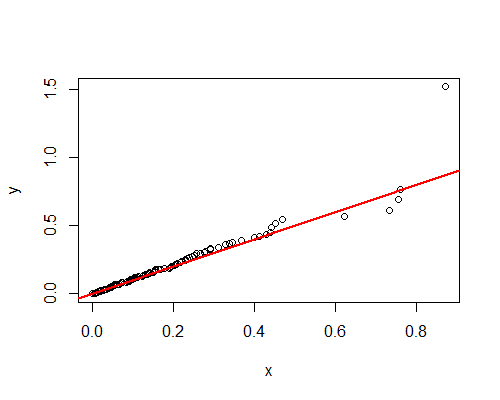
\includegraphics{ppapir.png}
\end{center}
\end{figure}

\subsection{}
Ve všech bodech diskutujte kvalitu vygenerovaných dat:
\\
Histogram hodnot $u$ neodpovídá příliš rovnoměrnému rozdělení, jelikož se v některých intervalech nachází více dat než v jiných. Tomu odpovídá i histogram dat $x$, jež vychází z transformace $u$ přes inverzi distribuční funkce exponenciálního rozdělení s parametrem $L$, ve kterém je vidět nečekaně vysoký počet hodnot $x$ větších než 0.4. Tyto nesrovnalosti jsou pravděpodobně způsobeny malým počtem vygenerovaných dat.
\\
Graf teoretické distribuční funkce ve třetí částí cvičení se velmi podobá empirické distribuční funkci. Menší shoda těchto funkcí se ukazuje pouze u vyšších hodnot x, kde jsou počty řídší.
\\
Ve čtvrté části cvičení by v ideálním případě hodnoty vykreslené funkcí $qqplot$ tvořily přímku, který je v grafu vykreslena červeně. Analogicky jako v předchozích cvičeních je to splněno pro nižší hodnoty $x$, kde je početnější zastoupení jednotlivých hodnot v jednotlivých intervalech. Naopak v právé části jsou odchylky větší - dat je málo a jsou náhodně generovaná, je tedy menší pravděpodobnost, že se setkají na zanesené přímce. 

\subsection{}
Extra 1/2 bodu: Použijte statistický test dobré shody (goodness of fit) pro ověření hypotézy $H_0$: Data pocházejí z rozdělení $Exp(L)$. Použijte některé z funkcí $chisq.test$, $ks.test$, nebo podobné.

\lstset{language = r, numbers=left, tabsize = 4, title=Řešení, basicstyle=\footnotesize}
\begin{lstlisting}[firstnumber=19]
# Vytvorim 10 binu po 0.1 od 0 do 1
breaks = c(seq(0, 1, by=.1))
# Priradim data do prislusnych intervalu
t = table(cut(x, breaks=breaks))
# Rozdily
d = diff(pexp(breaks, rate=L))
# Chi-kvadrat test dobre shody (porovnani rozdeleni do binu)
chisq.test(t, p=d, rescale.p=T)

	Chi-squared test for given probabilities

data:  t
X-squared = 13.123, df = 9, p-value = 0.1571
\end{lstlisting}
Z testu vyšlo, že data na 84 \% nepochazeji z rozdělení $Exp(L)$.


\vspace{1cm}
Zdroj - http://stackoverflow.com/questions/21655653/r-chi-square-goodness-of-fit-for-random-numbers-generated
\\
Vidíte do toho někdo víc?

%%
%% Úkol 2
%%

\section{Generování nehomogenního Poissonova procesu a grafické ověřování jeho rozdělení [2,5b]}
\subsection{}
Uvažujte příchod požadavků na webový server dle Poissonova procesu s proměnlivou intenzitou $lambda(t)$ příchodů za minutu
$$
\lambda(t) = 100 + 50exp\left\{-\frac{(t - 420)^2}{3600L}\right\}+100exp\left\{-\frac{L(-30L + t - 480)^2}{360000}\right\}
$$

Čas $t$ je měřen v minutách během 24 hodinového intervalu. Na začátku dalšího dne se intenzita periodicky opakuje, podobně jako v následující ilustraci.

%\begin{figure}[h]
%\begin{center}
%	\includegraphics[width=410px]{functiongraph.png}
%\end{center}
%\end{figure}

Pro první periodu $24*60$ minut můžeme intenzitu definovat jako funkci $lambda(t)$ v R pomocí

\lstset{title=Vstup, language=r}
\begin{lstlisting}
lambda = function(t) {
  100 + 50/exp((t - 420)^2/(3600*L)) + 100/exp((L*(t - 480 - 30*L)^2)/360000)
}
\end{lstlisting}

\subsection{}
Vygenerujte časy příchodů požadavků dle tohoto Poissonova procesu pro první den, čili pro první periodu $24*60$ minut. Zobrazte prvních $K*10$ příchodů na časové ose.

\vspace{1cm}
TODO

\subsection{}
Zobrazte četnosti příchodů pro celý den, t.j. pro všechy vygenerované příchody během peridy $24*60$ minut. Četnosti zobrazte spolu s grafem intenzity $lambda(t)$, podobně jako v následující ilustraci, kde červená křivka odpovídá předepsané intenzitě $lambda(t)$.
\\
Pro získání tohoto grafu jsme do proměnné 'h' uložili výsledek volání funkce hist() s parametrem plot=FALSE. Poté jsme zobrazili graf hodnot $h\$counts$ v bodech $h\$mids$. Parameter $breaks=$ funkce $hist()$ jsme zvolili tak, abychom počítali četnosti pro každou minutu. Více viz $help(hist)$.

\vspace{1cm}
TODO

\subsection{}
Diskutujte kvalitu vygenerovaných dat. Diskutujte efektivitu algoritmu z pohledu ztráty generovaných náhodných hodnot.
TODO

%%
%% Úkol 3
%%

\section{Simulace internetového obchodu s tokem nákupů dle nehomogenního Poissonova procesu  [1 bod]}
\subsection{}
Uvažujte internetový obchod s tokem objednávek dle nehomogenního Poissonova procesu z předchozího bodu. Ze všech zákazníků $K/(K+L)*100\%$ použije kurýrní službu, ostatní zvolí pro doručení objednávky státní poštu. Rozhodnutí o druzích doručení jsou náhodná a nezávislá mezi zákazníky i nezávislá od času zadání objednávky.

\vspace{1cm}
TODO

\subsection{}
Použijte časů příchodů Poissonova procesu vygenerovaných v předchozím bodě. Rozdělte tento proces na dva procesy:\newline
a) proces objednávek s použitím kurýrní služby a\newline
b) proces objednávek s použitím státní pošty.

\vspace{1cm}
TODO

\subsection{}
Zobrazte četnosti příchodů objednávek pro oba procesy pro celý den, t.j. během periody $24*60$ minut. Podobně jako v předchozím bodě, porovnejte četnosti s grafy intenzit $lambda\_kuryr(t)$ a $lambda\_pošta(t)$.

\vspace{1cm}
TODO

\end{document}